\hfill \newline
\phantom{ } We built the circuit according to the lab instruction, and recorded the following data.
\begin{table}[!htbp]
	\centering
	\caption{Amplitude and phase change of output signal of preamplifier}
	\begin{tabular}{lccccc}
		\toprule
		No &freq($\si{\hertz}$) &Amp\_in($\si{\milli\volt}$)&Amp\_out($\si{\volt}$)&Phase&gain(dB)\\
		\midrule
		1	&10		&104	&4.6	&180.00	&32.9145\\
		2	&20		&104	&4.6	&178.56	&32.9145\\
		3	&50		&108	&4.6	&183.60	&32.5867\\
		4	&100	&104	&4.6	&174.24	&32.9145\\
		5	&200	&106	&4.6	&178.56	&32.7490\\
		6	&500	&104	&4.6	&180.00	&32.9145\\
		7	&1000	&108	&4.9	&175.68	&33.1355\\
		8	&2000	&108	&4.9	&172.80	&33.1355\\
		9	&5000	&110	&4.7	&162.00	&32.6141\\
		\bottomrule
	\end{tabular}
	\label{tab:preamp}
\end{table}
\phantom{ } Then we plot the Bode plot in Excel according to [table\ref{tab:preamp}] in figure.

\begin{figure}[!htbp]
	\centering 
	\begin{framed}
		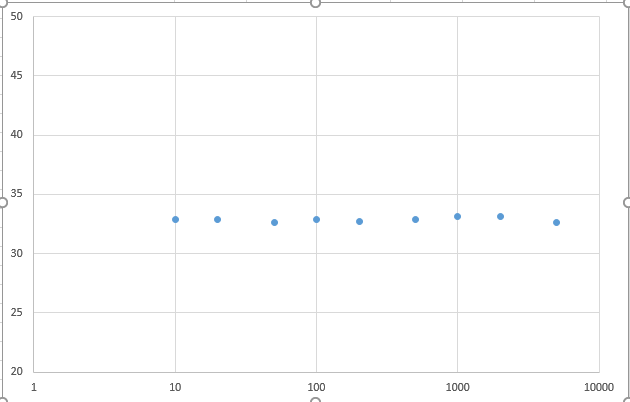
\includegraphics[width=\linewidth]{images/1_1.PNG} 
		\caption{Summing amplifier with potentiometers}
		\label{fig:101} 
	\end{framed}
\end{figure} 